%!TEX encoding = UTF-8 Unicode
\documentclass[french, a4paper, 12pt, twocolumn, landscape]{article}



%% Langue et compilation

\usepackage[utf8]{inputenc}
\usepackage[T1]{fontenc}
\usepackage[french]{babel}

%% LISTE DES PACKAGES

\usepackage{mathtools}     % package de base pour les maths
\usepackage{amsmath}       % mathematical type-setting
\usepackage{amssymb}       % symbols speciaux pour les maths
\usepackage{textcomp}      % symboles speciaux pour el text
\usepackage{gensymb}       % commandes generiques \degree etc...
\usepackage{tikz}          % package graphique
\usepackage{wrapfig}       % pour entourer a cote d'une figure
\usepackage{color}         % package des couleurs
\usepackage{xcolor}        % autre package pour les couleurs
\usepackage{pgfplots}      % pacakge pour creer des graph
\usepackage{epsfig}        % permet d'inclure des graph en .eps
\usepackage{graphicx}      % arguments dans includegraphics
\usepackage{pdfpages}      % permet d'insérer des pages pdf dans le document
\usepackage{subfig}        % permet de creer des sous-figure
\usepackage{pst-all}       % utile pour certaines figures en pstricks
\usepackage{lipsum}        % package qui permet de faire des essais
\usepackage{array}         % permet de faire des tableaux
\usepackage{multicol}      % plusieurs colonnes sur une page
\usepackage{enumitem}      % pro­vides user con­trol: enumerate, itemize and description
\usepackage{hyperref}      % permet de creer des hyperliens dans le document
\usepackage{lscape}        % permet de mettre une page en mode paysage
\usepackage{lmodern}       % permet d'avoir certains "fonts" de bonen qualite
\usepackage{fancyhdr}      % Permet de mettre des informations en hau et en bas de page      
\usepackage[framemethod=tikz]{mdframed} % breakable frames and coloured boxes
\usepackage[top=1.5cm, bottom=1.5cm, left=2.5cm, right=2.5cm]{geometry} % donne les marges
\usepackage[font=normalsize, labelfont=bf,labelsep=endash, figurename=Fig.]{caption} % permet de changer les legendes des figures
\usepackage{lewis}
\usepackage{bohr}
\usepackage{chemfig}
\usepackage{chemist}

%% LIBRAIRIES

\usetikzlibrary{plotmarks} % librairie pour les graphes
\usetikzlibrary{patterns}  % necessaire pour certaines choses predefinies sur tikz
\usetikzlibrary{shadows}   % ombres des encadres
\usetikzlibrary{backgrounds} % arriere plan des encadres


%% MISE EN PAGE

\pagestyle{fancy}     % Défini le style de la page

\renewcommand{\headrulewidth}{1pt}      % largeur du trait en haut de la page
\fancyhead[L]{Seconde générale}         % info coin haut gauche
\fancyhead[R]{Lycée Jean Guéhenno}  % info coin haut droit

% bas de la page
\renewcommand{\footrulewidth}{1pt}      % largeur du trait en bas de la page
\fancyfoot[L]{G. \bsc{LE DOUDIC}}  % info coin bas gauche
\fancyfoot[R]{TP 4 : Famille chimique}                         % info coin bas droit


\setlength{\columnseprule}{1pt} 
\setlength{\columnsep}{30pt}



%% NOUVELLES COMMANDES 

\DeclareMathOperator{\e}{e} % permet d'ecrire l'exponentielle usuellement


\newcommand{\gap}{\vspace{0.15cm}}   % defini une commande pour sauter des lignes
\renewcommand{\vec}{\overrightarrow} % permet d'avoir une fleche qui recouvre tout le vecteur
\newcommand{\bi}{\begin{itemize}}    % begin itemize
\newcommand{\ei}{\end{itemize}}      % end itemize
\newcommand{\bc}{\begin{center}}     % begin center
\newcommand{\ec}{\end{center}}       % end center
\newcommand\opacity{1}               % opacity 
\pgfsetfillopacity{\opacity}

\newcommand*\Laplace{\mathop{}\!\mathbin\bigtriangleup} % symbole de Laplace

\frenchbsetup{StandardItemLabels=true} % je ne sais plus

\newcommand{\smallO}[1]{\ensuremath{\mathop{}\mathopen{}o\mathopen{}\left(#1\right)}} % petit o

\newcommand{\cit}{\color{blue}\cite} % permet d'avoir les citations de couleur bleues
\newcommand{\bib}{\color{black}\bibitem} % paragraphe biblio en noir et blanc
\newcommand{\bthebiblio}{\color{black} \begin{thebibliography}} % idem necessaire sinon bug a cause de la couleur
\newcommand{\ethebiblio}{\color{black} \end{thebibliography}}   % idem
%%% TIKZ


%% COULEURS 


\definecolor{definitionf}{RGB}{220,252,220}
\definecolor{definitionl}{RGB}{39,123,69}
\definecolor{definitiono}{RGB}{72,148,101}

\definecolor{propositionf}{RGB}{255,216,218}
\definecolor{propositionl}{RGB}{38,38,38}
\definecolor{propositiono}{RGB}{109,109,109}

\definecolor{theof}{RGB}{255,216,218}
\definecolor{theol}{RGB}{160,0,4}
\definecolor{theoo}{RGB}{221,65,100}

\definecolor{avertl}{RGB}{163,92,0}
\definecolor{averto}{RGB}{255,144,0}

\definecolor{histf}{RGB}{241,238,193}

\definecolor{metf}{RGB}{220,230,240}
\definecolor{metl}{RGB}{56,110,165}
\definecolor{meto}{RGB}{109,109,109}


\definecolor{remf}{RGB}{230,240,250}
\definecolor{remo}{RGB}{150,150,150}

\definecolor{exef}{RGB}{240,240,240}

\definecolor{protf}{RGB}{247,228,255}
\definecolor{protl}{RGB}{105,0,203}
\definecolor{proto}{RGB}{174,88,255}

\definecolor{grid}{RGB}{180,180,180}

\definecolor{titref}{RGB}{230,230,230}

\definecolor{vert}{RGB}{23,200,23}

\definecolor{violet}{RGB}{180,0,200}

\definecolor{copper}{RGB}{217, 144, 88}

%% Couleur des ref

\hypersetup{
	colorlinks=true,
	linkcolor=black,
	citecolor=blue,
	urlcolor=black
		   }

%% CADRES


% %%%%%%%%%% DEFINITION
% \newmdenv[tikzsetting={fill=definitionf}, linewidth=2pt, linecolor=definitionl, outerlinewidth=0pt, innertopmargin=5pt, innerbottommargin=5pt, innerleftmargin=5pt, innerrightmargin=5pt, leftmargin=0pt]{definition}

% \newmdenv[ tikzsetting={drop shadow={ shadow xshift=1ex, shadow yshift=-0.5em, fill=definitiono, opacity=1, every shadow } }, outerlinewidth=2pt, outerlinecolor=white, linecolor=white, innertopmargin=0pt, innerbottommargin=0pt, innerleftmargin=0pt, innerrightmargin=0pt]{ombredef}


% %%%%%%%%%% THEOREME

% \newmdenv[tikzsetting={fill=theof}, linewidth=2pt, linecolor=theol, outerlinewidth=0pt, innertopmargin=5pt, innerbottommargin=5pt, innerleftmargin=5pt, innerrightmargin=5pt, leftmargin=0pt]{theo}

% \newmdenv[ tikzsetting={drop shadow={ shadow xshift=1ex, shadow yshift=-0.5em, fill=theoo, opacity=1, every shadow } }, outerlinewidth=2pt, outerlinecolor=white, linecolor=white, innertopmargin=0pt, innerbottommargin=0pt, innerleftmargin=0pt, innerrightmargin=0pt]{ombretheo}


% %%%%%%%%%% METHODE

% \newmdenv[tikzsetting={fill=metf}, linewidth=2pt, linecolor=metl, outerlinewidth=0pt, innertopmargin=5pt, innerbottommargin=5pt, innerleftmargin=5pt, innerrightmargin=5pt, leftmargin=0pt]{met}

% \newmdenv[ tikzsetting={drop shadow={ shadow xshift=1ex, shadow yshift=-0.5em, fill=meto, opacity=1, every shadow } }, outerlinewidth=2pt, outerlinecolor=white, linecolor=white, innertopmargin=0pt, innerbottommargin=0pt, innerleftmargin=0pt, innerrightmargin=0pt]{ombremet}



%%%%%%%%%%% RQ

\newmdenv[tikzsetting={fill=remf}, linewidth=2pt, linecolor=remf, outerlinewidth=0pt, innertopmargin=5pt, innerbottommargin=5pt, innerleftmargin=5pt, innerrightmargin=5pt, leftmargin=0pt]{remarque}

\newmdenv[ tikzsetting={drop shadow={ shadow xshift=1ex, shadow yshift=-0.5em, fill=remo, opacity=1, every shadow } }, outerlinewidth=2pt, outerlinecolor=white, linecolor=white, innertopmargin=0pt, innerbottommargin=0pt, innerleftmargin=0pt, innerrightmargin=0pt]{ombreremarque}

%%%%%%%%%%% Cadre pour le titre

\tikzset{every shadow/.style={opacity=1}}

\global\mdfdefinestyle{doc}{backgroundcolor=white, shadow=true, shadowcolor=propositiono, linewidth=1pt, linecolor=black, shadowsize=5pt}
\global\mdfdefinestyle{titr}{backgroundcolor=metf, shadow=true, shadowcolor=propositiono, linewidth=1pt, linecolor=black, shadowsize=5pt}
\global\mdfdefinestyle{theo}{backgroundcolor=theof, shadow=true, shadowcolor=theoo, linewidth=1pt, linecolor=theol, shadowsize=5pt}
\global\mdfdefinestyle{prop}{backgroundcolor=theof, shadow=true, shadowcolor=propositiono, linewidth=1pt, linecolor=theol, shadowsize=5pt}
\global\mdfdefinestyle{def}{backgroundcolor=definitionf, shadow=true, shadowcolor=definitiono, linewidth=1pt, linecolor=definitionl, shadowsize=5pt}
\global\mdfdefinestyle{histo}{backgroundcolor=histf, shadow=true, shadowcolor=propositiono, linewidth=1pt, linecolor=black, shadowsize=5pt}
\global\mdfdefinestyle{avert}{backgroundcolor=white, shadow=true, shadowcolor=averto, linewidth=1pt, linecolor=avertl, shadowsize=5pt}
\global\mdfdefinestyle{met}{backgroundcolor=metf, shadow=true, shadowcolor=meto, linewidth=1pt, linecolor=metl, shadowsize=5pt}
\global\mdfdefinestyle{rem}{backgroundcolor=metf, shadow=true, shadowcolor=meto, linewidth=1pt, linecolor=metf, shadowsize=5pt}
\global\mdfdefinestyle{exo}{backgroundcolor=exef, shadow=true, shadowcolor=propositiono, linewidth=1pt, linecolor=exef, shadowsize=5pt}
\global\mdfdefinestyle{not}{backgroundcolor=definitionf, shadow=true, shadowcolor=propositiono, linewidth=1pt, linecolor=black, shadowsize=5pt}
\global\mdfdefinestyle{proto}{backgroundcolor=protf, shadow=true, shadowcolor=proto, linewidth=1pt, linecolor=protl, shadowsize=5pt}

%%%%%%
\definecolor{cobalt}{rgb}{0.0, 0.28, 0.67}
\definecolor{applegreen}{rgb}{0.55, 0.71, 0.0}

\usepackage{tcolorbox}
  \tcbuselibrary{most}
  \tcbset{colback=cobalt!5!white,colframe=cobalt!75!black}



\newtcolorbox{definition}[1]{
	colback=applegreen!5!white,
  	colframe=applegreen!65!black,
	fonttitle=\bfseries,
  	title={#1}}
\newtcolorbox{Programme}[1]{
	colback=cobalt!5!white,
  	colframe=cobalt!65!black,
	fonttitle=\bfseries,
  	title={#1}}  

\newtcolorbox{Exercice}[1]{
  colback=cobalt!5!white,
  colframe=cobalt!65!black,
  fonttitle=\bfseries,
  title={#1}}  

  \newtcolorbox{Protocol}[1]{
  colback=cyan!5!white,
  colframe=cyan!65!black,
  fonttitle=\bfseries,
  title={#1}}  

\newtcolorbox{Resultat}[1]{
	colback=theof,%!5!white,
	colframe=theoo!85!black,
  fonttitle=\bfseries,
	title={#1}} 	


\def\width{12}
\def\hauteur{5}

\setlength{\parskip}{0pt}%
\setlength{\parindent}{18pt}


%% MODIFICATION DE CHAPTER  
\makeatletter
\def\@makechapterhead#1{%
  %%%%\vspace*{50\p@}% %%% removed!
  {\parindent \z@ \raggedright \normalfont
    \ifnum \c@secnumdepth >\m@ne
        \huge\bfseries \@chapapp\space \thechapter
        \par\nobreak
        \vskip 20\p@
    \fi
    \interlinepenalty\@M
    \Huge \bfseries #1\par\nobreak
    \vskip 40\p@
  }}
\def\@makeschapterhead#1{%
  %%%%%\vspace*{50\p@}% %%% removed!
  {\parindent \z@ \raggedright
    \normalfont
    \interlinepenalty\@M
    \Huge \bfseries  #1\par\nobreak
    \vskip 40\p@
  }}
  
  \newcommand{\isotope}[3]{%
     \settowidth\@tempdimb{\ensuremath{\scriptstyle#1}}%
     \settowidth\@tempdimc{\ensuremath{\scriptstyle#2}}%
     \ifnum\@tempdimb>\@tempdimc%
         \setlength{\@tempdima}{\@tempdimb}%
     \else%
         \setlength{\@tempdima}{\@tempdimc}%
     \fi%
    \begingroup%
    \ensuremath{^{\makebox[\@tempdima][r]{\ensuremath{\scriptstyle#1}}}_{\makebox[\@tempdima][r]{\ensuremath{\scriptstyle#2}}}\text{#3}}%
    \endgroup%
  }%

\makeatother

\usepackage{eurosym}
\usepackage{colortbl}
% \onehalfspacing
%%
%% DEBUT DU DOCUMENT
%%
\begin{document}


%%%%%%

\titre{Chapitre 10 : Solutions aqueuses}

\doc{1}{Bulletin officiel}{
\begin{center}
	% 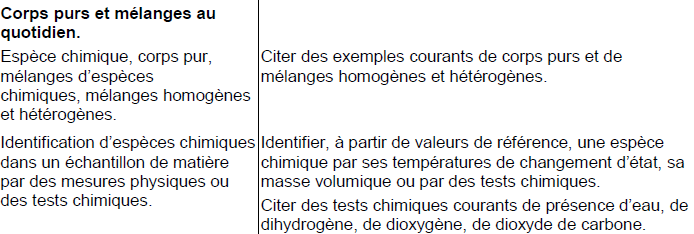
\includegraphics[width=.95\textwidth]{BO1.png}
	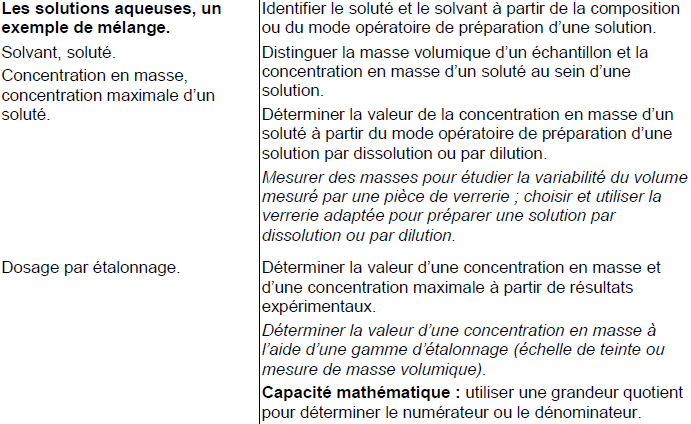
\includegraphics[width=.95\textwidth]{BO.png}
\end{center}
}


\doc{2}{Exercices dans le livre scolaire}{
		\begin{enumerate}
			\item Compétence de base : exercice 5, 7, 9 page 48
			\item Pour confirmer  : exercice 12,  13, 16 page 49
			\item Parcours expert exercice 21 page 51
		\end{enumerate}
}\vspace{1cm}
	\noindent \textbf{Quiz sur les solutions aqueuses}
\begin{center}
	\begin{minipage}{.12\textwidth}
		\centering
		
\includegraphics[width=.5\textwidth]{Quiz1.png}
		
		Quiz 1 - Les solutions aqueuses : \url{https://forms.office.com/r/4T8uu5T9fr?origin=lprLink}
	\end{minipage}\hspace{.5cm}
	\begin{minipage}{.12\textwidth}
		\centering
		
\includegraphics[width=.5\textwidth]{Quiz2.png}

		Quiz 2 - Concentration massique : \url{https://forms.office.com/r/9fY0GJnYxJ?origin=lprLink}
	\end{minipage}\hspace{.5cm}
\begin{minipage}{.12\textwidth}
			\centering
			
\includegraphics[width=.5\textwidth]{Quiz3.png}
	
			Quiz 3 - Préparation d'une solution : \url{https://forms.office.com/r/deBzELcd2Y?origin=lprLink}
		\end{minipage}
\end{center}


\section*{Introduction}

L'eau de mer, la plupart de boissons et nombre de solutions fréquemment utilisées en chimie sont des exemples de solutions aqueuses. Dans ce chapitre, on s'intéresse à ces solutions ainsi qu'à leur préparation. 

\begin{figure}[ht]
	\centering
	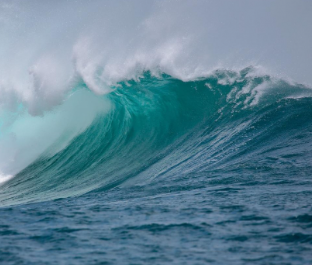
\includegraphics[width=.2\textwidth]{EauDeMer.png}\hspace{1cm}
	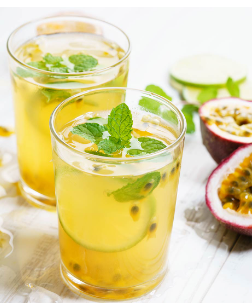
\includegraphics[width=.15\textwidth]{limonade.png}
	\caption{À gauche de l'eau de mer, à droite une limonade rafraîchissante}
\end{figure}
\section{La solution aqueuse, un exemple de mélange homogène}

\begin{definition}{Définition 1 - Solution}

	Un solution  est un \textbf{mélange}. Ce mélange est constitué : \medskip 

	\begin{itemize}
	\item d'un \textbf{solvant} : composant majoritaire du mélange;
	\item d'un \textbf{soluté} : espèce chimique dispersée dans le solvant.
	\end{itemize}
	
\end{definition}

\begin{figure}[ht]
	\centering
	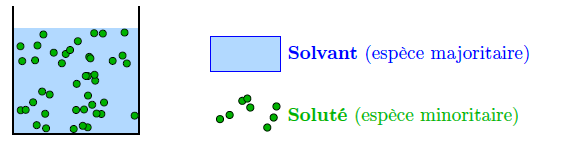
\includegraphics[width=.5\textwidth]{solution.png}
\end{figure}

Dans le cas où le solvant est l'eau, on parlera de solution \textbf{aqueuse}.

\exo{1}{Cuisson des pâtes}{Afin de cuire des pâtes, on prépare une solution d'eau salée (($\rm Na^+_{\rm (aq)}, Cl^-_{\rm (aq)}$) en solution).

\begin{itemize}
\item \analyser Identifier le solvant et le soluté. Comment appelle-t-on ce type de solution ?\medskip

\textbf{Solution :} Le solvant est l'eau, le soluté est le sel. Il s'agit d'une solution aqueuse car le solvant est de l'eau.

\item \analyser Le soluté est-il ionique ou moléculaire ? \medskip

\textbf{Solution :} Le soluté est ionique car le sel dissous dans l'eau se sépare en deux ions, les ions sodium et les ions chlorures.

\end{itemize}
}	

\section{Concentration massique}
Lorsque l'on prépare une solution, on peut \textbf{faire varier la quantité de soluté que l'on dissout} par unité de volume. Par exemple, il est possible de préparer un café très sucré ou peu sucré. La \textbf{contentration massique} est une grandeur permettant de quantifier cela.

\begin{definition}{Définition 2 - Concentration massique (ou titre massique)}
	\medskip
	La concentration massique d'un soluté est la masse $m$ de soluté dissous dans un volume $V$ de la solution: 

	$$C_{\rm m} \footnote{Parfois noté $\gamma$ ou $t_{\rm m}$}= \dfrac{m}{V}$$

	$C_{\rm m}$ est exprimé en \textbf{$g\cdot L^{-1}$}, m en \textbf{$g$} et V en \textbf{$L$}.
\end{definition}

\avert{}{Concentration massique et masse volumique}{

La concentration en masse d'un soluté, notée $C_{\rm m}$ , représente la masse m de soluté dissous par litre de solution . La masse volumique $\rho$ d'un corps est la masse de ce corps par unité de volume. 

}

\exo{2}{Café sucré}{\realiser On a dissous dans un café un carré de sucre de masse $m_s=5$ g. Le volume de la boisson est alors de 200 mL. Quelle est sa concentration massique en sucre ? \medskip

\textbf{Solution} : Par définition $C_{\rm m} = \dfrac{m}{V} = \dfrac{5~(g)}{200\times 10^{-3}~(L)} = 25~\rm g\cdot L^{-1}.$}

\section{Préparation des solutions}

Il existe principalement deux méthodes pour préparer des solutions : par \textbf{dissolution} d'un soluté ou par \textbf{dilution} d'une solution déjà existante.\medskip

De manière générale, la préparation de solutions recquiert l'utilisation de \textbf{verrerie de précision}.

\subsection{Préparation par dissolution}

\begin{definition}{Définition 4 - Dissolution}
	La dissolution est la dispersion d'un soluté dans un solvant.
\end{definition}

La marche 1a suivre pour préparer une solution par dissolution est la suivante : 

\begin{figure}[ht]
	\centering
	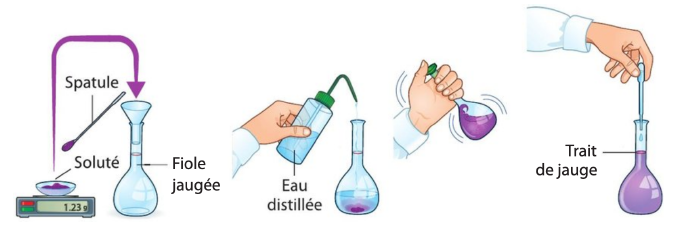
\includegraphics[width=\linewidth]{Dissolution.png}
\end{figure}

\begin{Proposition}{Propriété 1 - Masse de soluté à dissoudre}
	La masse de soluté prélevée se retrouve toujours dans la solution préparée. On dit que la masse est conservée:

	$$m_{\rm soluté~pesé} = m_{\rm soluté~en~solution} = C_{m_{\rm solution}}V_{\rm solution}$$
\end{Proposition}

\subsection{Dilution}

\begin{definition}{Définition 5 - Dilution}

	Une dilution est la diminution de la concentration d'une solution par ajout de solvant sans ajout de soluté.
	
\end{definition}

\begin{Proposition}{Propriété 2 - Relation fondamentale des dilutions}
	La masse de soluté prélevée dans la solution mère est égale à la masse de soluté contenue dans la solution fille : $m_{\rm mère} = m_{\rm fille}$. On a donc \dotfill \vspace{1cm}

	$$\dfrac{C_{\rm m_{\rm mère}}}{C_{\rm m_{\rm fille}}}=\dfrac{V_{\rm mère}}{V_{\rm fille}} = F = \text{ facteur de dilution}$$
\end{Proposition}
% \clearpage

La marche à suivre pour réaliser une dilution est la suivante :
\begin{figure}[ht]
	\centering
	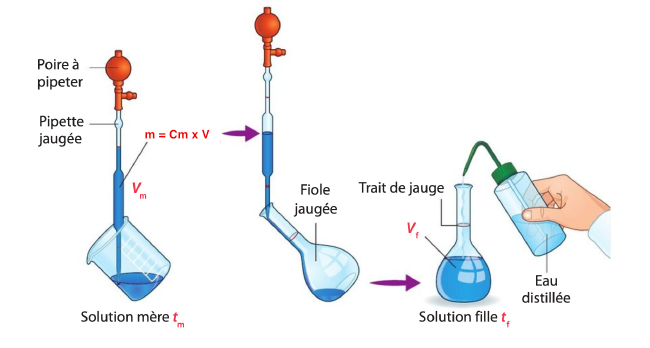
\includegraphics[width=1\linewidth]{Dilution.png}
\end{figure}

% \exo{3}{Bouillie bordelaise}{Afin de traiter des plants de tomates contre des champignons, on souhaite préparer 2,0 L de solution de sulfate de cuivre concentrée à 150 $\rm g\cdot L^{-1}$. 

% \realiser Quelle masse de sulfate de cuivre anhydrde doit-on dissoudre ? \vspace{2cm}}

\section{Déterminer une concentration : le dosage par étalonnage}

\textbf{Doser} une solution signifie \og{}\textbf{déterminer sa concentration ou sa quantité de matière}\fg{}. Il est possible de doser une espèce $E$ dans une solution par \textbf{étalonnage} :

\begin{enumerate}
	\item On prépare une gamme de solutions de concentrations en $E$ connues. Ce sont les solutions \textbf{étalons};
	\item On compare une grandeur physique\footnote{comme la couleur} de la solution à doser à ces solutions étalons. On peut ainsi en déduire un encadrement de sa concentration.
\end{enumerate}

\begin{figure}[ht]
	\centering
	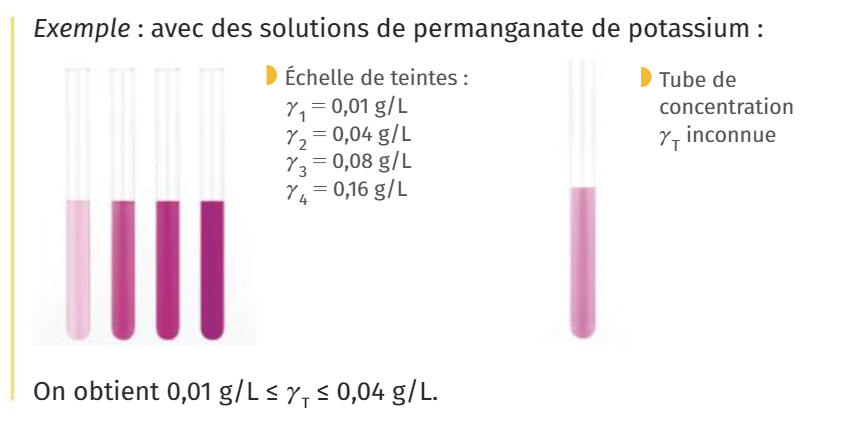
\includegraphics[width=.5\textwidth]{dosageparetalonnag.png}
\end{figure}

Si la solution est incolore, on peut mesurer une grandeur caractéristique, telle que la masse volumique et comparer la valeur obtenue à celle des solutions étalons.
\end{document}

%%
%% FIN DU DOCUMENT
%%
